\documentclass[UTF8,zihao=-4,fontset=windows]{ctexart}

% 页面与版式
\usepackage[a4paper,top=3.0cm,bottom=2.5cm,left=2.5cm,right=2.5cm,headheight=15pt,headsep=0.5cm,footskip=1.0cm]{geometry}
\usepackage{fontspec}
\usepackage{graphicx}
\usepackage{array}
\usepackage{tabularx}
\usepackage{longtable}
\usepackage{multirow}
\usepackage{booktabs}
\usepackage{amsmath,amssymb}
\usepackage{caption}
\usepackage{fancyhdr}
\usepackage{titlesec}
\usepackage{tocloft}
\usepackage{indentfirst}
\usepackage{enumitem}
\usepackage{float}
\usepackage{ifthen}
\usepackage{etoolbox}

% 参考文献上标
\let\oldcite\cite
\renewcommand{\cite}[1]{\textsuperscript{\oldcite{#1}}}

\IfFontExistsTF{Times New Roman}{\setmainfont{Times New Roman}}{\setmainfont{Tinos}}

% 基本段落：正文宋体小四号，固定行距约 20 磅，段前段后 0，首行缩进 2 字符。
\setlength{\parindent}{2em}
\setlength{\parskip}{0pt}
\renewcommand{\baselinestretch}{1.38}
\raggedbottom
\setlist{nosep}

% 作品信息：集中改这里即可。
\newcommand{\contestName}{第六届四川省大学生生物医学工程创新设计竞赛}
\newcommand{\templateName}{第一轮作品报告}
\newcommand{\reportTitle}{基于深度迁移学习与手工特征融合的脑电情绪识别方法}
\newcommand{\reportTitleShort}{基于深度迁移学习与手工特征融合的脑电情绪识别方法}
\newcommand{\workID}{202015}
\newcommand{\studentType}{本科生}
\newcommand{\trackName}{医学人工智能}
\newcommand{\groupName}{命题项目组}
\newcommand{\reportDate}{2026 年 5 月}

% 页眉页脚
\pagestyle{fancy}
\fancyhf{}
\renewcommand{\headrulewidth}{0.4pt}
\renewcommand{\footrulewidth}{0pt}
\fancyhead[L]{\zihao{5}\songti \reportTitleShort}
\fancyhead[R]{\zihao{5}\songti \leftmark}
\fancyfoot[C]{\zihao{5}\thepage}

\newcommand{\frontHeader}[1]{%
  \fancyhf{}%
  \renewcommand{\headrulewidth}{0.4pt}%
  \fancyhead[L]{\zihao{5}\songti \reportTitle}%
  \fancyhead[R]{\zihao{5}\songti #1}%
  \fancyfoot[C]{\zihao{5}\thepage}%
  \fancypagestyle{plain}{%
    \fancyhf{}%
    \renewcommand{\headrulewidth}{0.4pt}%
    \fancyhead[L]{\zihao{5}\songti \reportTitle}%
    \fancyhead[R]{\zihao{5}\songti #1}%
    \fancyfoot[C]{\zihao{5}\thepage}%
  }%
}
\newcommand{\mainHeader}{%
  \fancyhf{}%
  \renewcommand{\headrulewidth}{0.4pt}%
  \fancyhead[L]{\zihao{5}\songti \reportTitleShort}%
  \fancyhead[R]{\zihao{5}\songti \leftmark}%
  \fancyfoot[C]{\zihao{5}\thepage}%
  \fancypagestyle{plain}{%
    \fancyhf{}%
    \renewcommand{\headrulewidth}{0.4pt}%
    \fancyhead[L]{\zihao{5}\songti \reportTitleShort}%
    \fancyhead[R]{\zihao{5}\songti \leftmark}%
    \fancyfoot[C]{\zihao{5}\thepage}%
  }%
}

% 一级章节按模板习惯另起新页，并将页眉右侧同步为当前章标题。
\pretocmd{\section}{\clearpage}{}{}
\renewcommand{\sectionmark}[1]{\markboth{\thesection\quad #1}{}}

% 标题格式：一级三号黑体居中；二级小三号黑体；三级四号黑体。
\titleformat{\section}{\centering\heiti\zihao{3}}{\thesection}{1em}{}
\titleformat{\subsection}{\heiti\zihao{-3}}{\thesubsection}{0.75em}{}
\titleformat{\subsubsection}{\heiti\zihao{4}}{\thesubsubsection}{0.75em}{}
\titlespacing*{\section}{0pt}{0pt}{1.0\baselineskip}
\titlespacing*{\subsection}{0pt}{1.0\baselineskip}{0.3\baselineskip}
\titlespacing*{\subsubsection}{0pt}{0.8\baselineskip}{0.2\baselineskip}

% 目录格式：五号字，点线。
\renewcommand{\contentsname}{目\hspace{1em}录}
\renewcommand{\cfttoctitlefont}{\hfill\heiti\zihao{3}}
\renewcommand{\cftaftertoctitle}{\hfill}
\setlength{\cftbeforetoctitleskip}{0pt}
\setlength{\cftaftertoctitleskip}{1.0\baselineskip}
\renewcommand{\cftsecfont}{\heiti\zihao{5}}
\renewcommand{\cftsecpagefont}{\heiti\zihao{5}}
\renewcommand{\cftsubsecfont}{\songti\zihao{5}}
\renewcommand{\cftsubsecpagefont}{\songti\zihao{5}}
\renewcommand{\cftsubsubsecfont}{\songti\zihao{5}}
\renewcommand{\cftsubsubsecpagefont}{\songti\zihao{5}}
\setlength{\cftsecindent}{0em}
\setlength{\cftsubsecindent}{2em}
\setlength{\cftsubsubsecindent}{4em}
\setlength{\cftbeforesecskip}{0pt}
\renewcommand{\cftdotsep}{1.2}

% 图表与公式编号：按章编号，如图 3.3、表 3.2。
\numberwithin{equation}{section}
\numberwithin{figure}{section}
\numberwithin{table}{section}
\captionsetup{font={small},labelfont={normalfont},labelsep=space,justification=centering}
\captionsetup[table]{position=top}
\captionsetup[figure]{position=bottom}
\renewcommand{\figurename}{图}
\renewcommand{\tablename}{表}

% 封面
\newcommand{\makeReportCover}{%
\newgeometry{top=2.54cm,bottom=2.54cm,left=3.17cm,right=3.17cm}
\thispagestyle{empty}
\begin{center}
  {\songti\zihao{-2}\contestName}\par
  \vspace{0.8cm}
  {\songti\zihao{-2}\templateName}\par
  \vspace{6.5cm}
  {\heiti\zihao{1}\reportTitle}\par
  \vspace{2.5cm}
  % \includegraphics[width=2.55cm]{bme_logo.jpeg}  % logo file not provided\par
  \vfill
  \hspace{1cm}\begin{minipage}{7.5cm}
    \songti\zihao{3}
    \makebox[6em][s]{作品ID号}： \workID\par\vspace{0.45cm}
    \makebox[6em][s]{参赛学生类型}： \studentType\par\vspace{0.45cm}
    \makebox[6em][s]{参加赛道}： \trackName\par\vspace{0.45cm}
    \makebox[6em][s]{组别}： \groupName\par
  \end{minipage}\par
  \vspace{1.45cm}
  {\songti\zihao{3}\reportDate}\par
\end{center}
\clearpage
\restoregeometry
}

% 内容完整性自查表
\newcommand{\makeChecklist}{%
\thispagestyle{empty}
\begin{center}

\vspace{1.0cm}
{\heiti\zihao{3} 内容完整性自查表}\par
\end{center}
\vspace{0.4cm}
\noindent{\songti\bfseries 说明：}\par
\noindent{\songti\bfseries 1. 命题组参赛作品请根据命题文件规定或要求的指标填写；}\par
\noindent{\songti\bfseries 2. 自选组参赛作品请根据实际参赛作品完成情况填写。}\par
\vspace{0.5cm}
\renewcommand{\arraystretch}{1.2}
\begin{longtable}{|>{\centering\arraybackslash}p{2.6cm}|>{\centering\arraybackslash}p{3.6cm}|>{\centering\arraybackslash}p{3.2cm}|>{\centering\arraybackslash}p{5.0cm}|}
\hline
\parbox[c][1.6cm][c]{2.6cm}{\centering\renewcommand{\baselinestretch}{1.0}\selectfont 评估维度} &
\parbox[c][1.6cm][c]{3.6cm}{\centering\renewcommand{\baselinestretch}{1.0}\selectfont 任务或技术指标名称} &
\parbox[c][1.6cm][c]{3.2cm}{\centering\renewcommand{\baselinestretch}{1.0}\selectfont 完成效果} &
\parbox[c][1.6cm][c]{5.0cm}{\centering\renewcommand{\baselinestretch}{1.0}\selectfont 呈现方式（报告中的章节、页码，或测试报告、实物、视频等）} \\
\hline
\multirow{3}{*}{\parbox{2.4cm}{\centering 算法设计的\\创新性}} &
  1. 跨数据集迁移学习策略（DEAP预训练+微调） &
  已实现，DEAP上EEGNet达79.10\% &
  第2.4.2节（第10--11页） \\
\cline{2-4}
&
  2. 手工特征与深度学习异构融合 &
  软投票融合达64.26\%，超两个单独模型 &
  第2.5节（第11--12页）；表3.1 \\
\cline{2-4}
&
  3. 模型容量-泛化关系的对照设计 &
  验证了小样本下容量控制优于架构精细化的判断 &
  第2.4.2节、第3.3.2节；图3.5 \\
\hline
\multirow{4}{*}{\parbox{2.4cm}{\centering 方案与模型\\的完整性}} &
  4. 数据预处理管线（滤波/分段/标准化） &
  竞赛与DEAP数据统一预处理 &
  第2.2节（第3--8页） \\
\cline{2-4}
&
  5. 手工特征工程（DE/PSD/Hjorth共390维） &
  覆盖频域能量、频域结构和时域形态 &
  第2.3节（第8--9页） \\
\cline{2-4}
&
  6. 深度学习模型训练与对比（EEGNet/TSception） &
  EEGNet 63.96\%，TSception 53.35\% &
  第2.4.1节（第10页）；表3.1 \\
\cline{2-4}
&
  7. 消融实验验证各组件贡献 &
  预训练、容量、特征贡献三项消融全部完成 &
  第3.3节（第14--18页）；图3.4--3.8 \\
\hline
\multirow{3}{*}{\parbox{2.4cm}{\centering 本地可验证\\的性能}} &
  8. 跨被试泛化：5折GroupKFold按被试划分 &
  训练集与验证集无同源被试 &
  第3.1节（第13页） \\
\cline{2-4}
&
  9. 性能水平：5折CV准确率与标准差 &
  最优融合64.26\%±1.45\%，全部模型完整报告 &
  表3.1；图3.3 \\
\cline{2-4}
&
  10. 稳定性：跨折波动范围与训练曲线 &
  5折标准差1.45\%--2.87\%，训练/验证曲线收敛正常 &
  图3.6--3.7 \\
\hline
\multirow{2}{*}{其他} &
  测试集推理与提交文件生成 &
  10名被试×8 trial，含4正4负先验校准 &
  第3.4节；submission.xlsx \\
\cline{2-4}
&
  全流程代码实现 &
  可复现：预处理、特征提取、训练、评估、推理 &
  src/；checkpoints/ \\
\hline
\end{longtable}
\clearpage
}

% 摘要页
\newcommand{\makeAbstractPage}{%
\frontHeader{摘要}
\phantomsection
\addcontentsline{toc}{section}{摘要}
\begin{center}
{\heiti\zihao{3} 摘\hspace{2em}要}
\end{center}
\vspace{0.8cm}\par
脑电情绪识别在小样本、高维度、跨被试场景下面临严重的过拟合与泛化困难。本文提出一种深度迁移学习与手工特征融合的脑电情绪二分类方案。在深度学习管线中，以仅2,834参数的EEGNet为核心模型，利用DEAP公开数据集进行预训练后在竞赛数据上微调，并与3,111,106参数的TSception模型构成容量对照。在手工特征管线中，提取微分熵、功率谱密度和Hjorth参数共390维特征，输入LightGBM梯度提升决策树进行分类。两条管线通过软投票进行异构融合。所有实验在5折GroupKFold按被试划分的交叉验证下评估，确保同一被试的数据不被拆分至训练集和验证集两侧。实验结果表明：轻量级EEGNet达到63.96\%的5折平均准确率，而大容量TSception仅53.35\%，验证了在小样本条件下模型容量控制比架构精细化更为关键的判断；手工特征结合LightGBM达到62.19\%；两者软投票融合达到最高的64.26\%。DEAP预训练在本实验条件下未带来统计显著的性能增益，揭示了源域与目标域之间范式差异对迁移学习的制约。特征重要性分析显示，$\gamma$和$\alpha$波段的微分熵是最具区分力的特征，顶颞区电极（通道18、12、17、22）为情绪分类的关键位点，与神经科学文献独立一致。

\vspace{2\baselineskip}
\noindent{\heiti 关键词：}{\songti 脑电情绪识别；迁移学习；EEGNet；LightGBM；微分熵}
\clearpage
}

% 三线表、四线表辅助命令
\newcommand{\threelinetabletop}{\toprule}
\newcommand{\threelinetablemid}{\midrule}
\newcommand{\threelinetablebottom}{\bottomrule}

\begin{document}
\songti\zihao{-4}

\makeReportCover
\makeChecklist

% 前置部分：罗马页码，从摘要开始。
\pagenumbering{Roman}
\setcounter{page}{1}
\makeAbstractPage

\frontHeader{摘要}
\tableofcontents
\clearpage

% 正文：阿拉伯页码，从 1 开始。
\mainHeader
\pagenumbering{arabic}
\setcounter{page}{1}

% =================================================================
% 第 1 章：作品概述
% =================================================================
\section{作品概述}

\subsection{背景及意义}

情绪识别在人机交互、心理健康评估和医学诊断等领域具有重要应用价值。与传统基于面部表情或语音的情绪识别方法相比，脑电信号直接从大脑皮层采集，能够更客观地反映人的真实情感状态，难以被主观掩饰，被誉为情绪识别的``金标准''。

然而，基于脑电的情绪识别面临三大核心挑战：(1) \textbf{高维度低样本量}：单次EEG记录包含30通道×数千时间点的高维数据，但可用被试数量通常较少（本赛题60人），深度学习模型极易过拟合；(2) \textbf{跨被试泛化困难}：不同被试的脑电信号存在巨大的个体差异（电极位置、颅骨厚度、基线脑活动等），同一模型在不同被试上的表现可能大幅波动；(3) \textbf{信号信噪比低}：EEG信号易受眼电、肌电、运动伪迹等噪声干扰，情绪相关的微弱有用信号往往被淹没。

本作品围绕上述挑战，设计并实现了一套\textbf{深度迁移学习与手工特征融合}的脑电情绪识别方案。

\subsection{研究基础}

随着深度学习技术的快速发展，卷积神经网络和图神经网络已被广泛应用于脑电情绪识别领域。Lawhern等学者提出了EEGNet\cite{eegnet}，通过深度可分离卷积将时域滤波与空域滤波解耦，在仅需2,500个参数的轻量结构下实现了跨被试运动想象分类，验证了参数高效模型在脑电小样本场景下的可行性。Ding等学者在此基础上提出了专门面向情绪识别的TSception\cite{tsception}模型，引入了多尺度动态时间层和左右脑非对称空间层，分别在时域捕捉不同频段的EEG动态特征、在空域利用情绪处理的半球不对称性进行编码，在DEAP\cite{deap}数据集上取得了显著的性能提升。但TSception模型参数量达311万，其在大规模公开数据集上的优势能否迁移至仅有数十名被试的小规模竞赛数据，仍缺乏系统性验证。

在脑电特征工程方面，Duan等学者的研究证实微分熵（Differential Entropy, DE）是脑电情绪识别中最优的单类频域特征，其在高频段（$\beta$和$\gamma$波段）的判别能力尤为突出。功率谱密度、Hjorth参数等时频域特征与DE组合后的多维特征向量，已被多项研究验证为有效的脑电情绪表征方案。在分类器选择上，Ke等学者提出的LightGBM\cite{lightgbm}采用leaf-wise决策树生长策略和基于梯度的单边采样（GOSS），在保证分类精度的同时显著降低了训练时间与内存开销，尤其适合多维特征的小样本分类任务。

在跨被试泛化评估方法方面，传统研究常采用被试内随机划分策略进行评估，但近年来的研究表明该策略将同一被试的不同trial分散至训练集和验证集，导致模型实际学习的是被试身份而非情绪状态，产生严重的数据泄露和虚假高分。采用严格的留一被试（LOSO）或GroupKFold按被试划分策略已成为脑电情绪识别领域的共识性评估范式。

总体而言，现有研究多聚焦于SEED（62通道、15人）和DEAP（32通道、32人）等公开数据集的评估，对通道数更少（30通道）、被试异质性更高（混合健康对照与抑郁症患者）的小规模竞赛数据场景缺乏验证。同时，深度学习模型在该场景下是否优于基于手工特征的传统机器学习方法尚无定论。以上现状构成了本项目的研究基础。

\subsection{研究目标}

本项目旨在构建一种适用于小样本场景的跨被试脑电情绪识别方法，具体研究目标如下：

\begin{enumerate}[label={(\arabic*)}, labelindent=2em, leftmargin=4.5em, itemindent=0pt, labelsep=0.5em]
    \item 在严格的跨被试验证条件下，实现显著超过随机基线的稳定分类准确率，为30通道60人被试规模的脑电情绪识别提供可靠的基准模型。
    \item 探索跨数据集迁移学习对小样本脑电分类的实际增益：利用DEAP公开数据集对EEGNet、TSception等深度模型进行预训练后迁移至竞赛数据，系统评估不同模型架构在迁移学习中的表现差异。
    \item 对比深度学习端到端学习与传统手工特征方法（DE、PSD、Hjorth特征结合LightGBM分类器）在小样本跨被试场景下的性能差异，为脑电情绪识别的工程实践提供方法选择参考。
    \item 验证EEGNet等轻量级深度学习模型与LightGBM传统机器学习模型进行异构软投票融合的可行性，探索两种完全不同学习范式之间的互补潜力。
\end{enumerate}

% =================================================================
% 第 2 章：作品方案设计及实现
% =================================================================
\section{作品方案设计及实现}

\subsection{技术路线概述}

本方案的整体技术路线如图\ref{fig:pipeline}所示，分为如下三个阶段：

\textbf{第一阶段，数据预处理与公开数据集预训练。} 竞赛数据集（60名被试，30通道，250Hz采样率）与DEAP公开数据集（32名被试，32通道，128Hz采样率）分别进行通道对齐、带通滤波（0.5--50Hz）、滑动窗分段（10秒窗口，2500采样点）和Z-score标准化，得到统一格式的EEG trial。在此基础上，利用DEAP数据集分别对EEGNet和TSception两个深度模型进行预训练，学习EEG情绪的通用时空表征。预训练后的模型权重作为后续微调的初始参数。同时，从标准化后的竞赛EEG trial中提取微分熵（DE，5频段×30通道=150维）、功率谱密度（PSD，5频段×30通道=150维）和Hjorth参数（Activity/Mobility/Complexity×30通道=90维），构成390维手工特征向量，供LightGBM模型使用。

\textbf{第二阶段，模型训练与交叉验证。} 本方案设计了\textbf{两主线一对照}的模型训练架构：

\begin{enumerate}[label={(\arabic*)}, labelindent=2em, leftmargin=4.5em, itemindent=0pt, labelsep=0.5em]
    \item \textbf{主线A：深度学习端到端路线}。以EEGNet为核心模型，直接接收预处理后的原始EEG信号（30通道×2500采样点），通过时间卷积、空间深度可分离卷积和可分离卷积三层结构提取层次化时空特征，经全连接层输出二分类结果。EEGNet总参数量仅2,834个，天然适配小样本场景。作为对照，同时训练311万参数量的TSception模型，用于验证模型复杂度与泛化能力的关系。
    \item \textbf{主线B：手工特征与机器学习路线}。基于390维手工特征向量，使用LightGBM梯度提升决策树进行分类。LightGBM采用leaf-wise生长策略和GOSS采样，训练速度快且内置特征重要性排序，为模型决策提供可解释性。
    \item \textbf{迁移学习对照实验}：对EEGNet和TSception分别设置``从零训练''和``DEAP预训练+微调''两种训练模式。微调模式下加载阶段一的DEAP预训练权重，以更低的学习率（$1\times10^{-4}$）和更高的权重衰减（$1\times10^{-3}$）在竞赛数据上继续训练，以探究跨数据集迁移学习的实际增益。
\end{enumerate}

所有模型训练和评估均采用\textbf{5折GroupKFold按被试划分}的交叉验证策略，即将60名被试随机分为5组，每折以4组（48人）的数据训练、1组（12人）的数据验证。关键约束是同一被试的所有trial被完整地分入同一折，杜绝被试信息跨折泄露，确保验证分数真实反映模型的跨被试泛化能力，而非对被试身份的过拟合。每折报告准确率，以5折均值±标准差作为最终评价指标。

\textbf{第三阶段，模型融合与测试集推理。} 训练完成后，将主线A的最优模型（EEGNet）与主线B的最优模型（LightGBM）进行异构软投票融合：对同一测试trial，两个模型分别输出积极类别的预测概率，取算术平均作为融合概率，以0.5为阈值进行二分类判别。此外，利用测试集中每名被试恰好包含4段积极视频和4段中性视频的先验信息，对每名被试的8个trial预测概率进行排序，取概率最高的4个trial标为积极，其余标为中性，进一步提升预测合理性。最终输出格式为包含user\_id、trial\_id和Emotion\_label的submission.xlsx文件。

\begin{figure}[H]
\centering
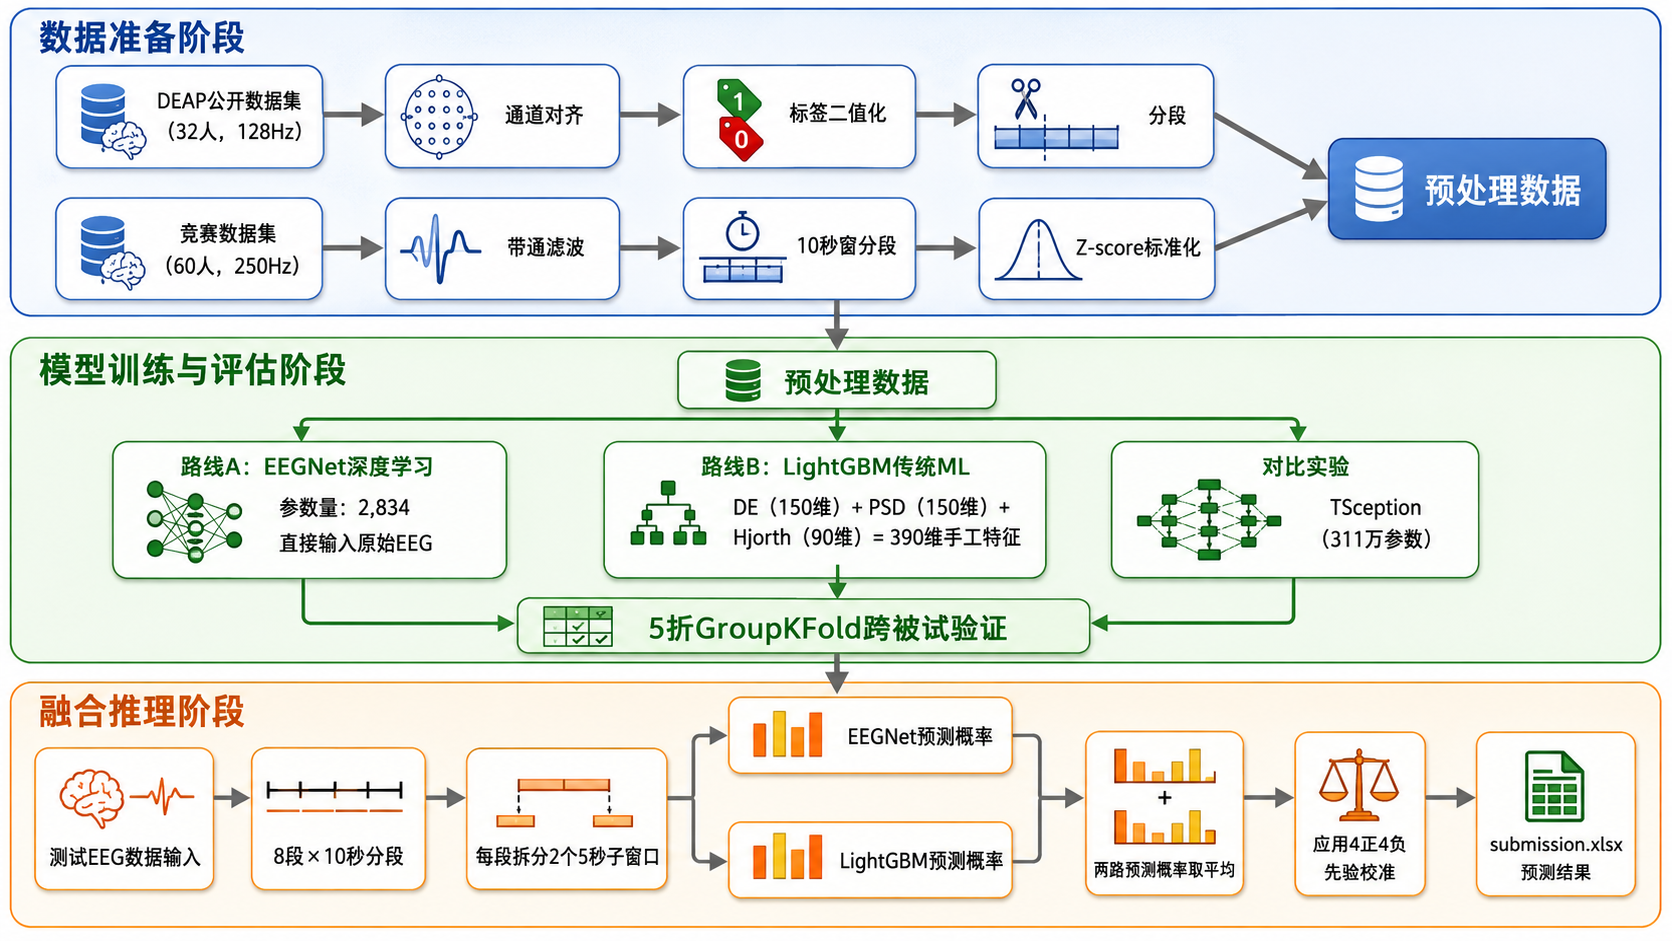
\includegraphics[width=0.85\textwidth]{figures/papiline.png}
\caption{总体技术路线流程图}
\label{fig:pipeline}
\end{figure}

\subsection{数据预处理}

\subsubsection{数据集描述}

本方案涉及两个脑电数据集的预处理与格式对齐：竞赛数据集与DEAP公开数据集。

竞赛数据集的训练集包含60名被试（40名健康对照HC + 20名抑郁症患者DEP），每名被试在两种情绪状态（中性、积极）下分别记录了30通道的脑电信号，每段记录为50,000个连续采样点（250Hz×4段视频×50秒），原始记录以A2（右耳垂）为物理参考电极，组委会在预处理中已将其转换为平均参考（每个采样点减去30通道的瞬时平均值），并完成0.01Hz高通滤波去基线漂移及工频陷波等预处理。测试集包含10名被试（5名HC + 5名DEP），每名被试包含8段情绪视频对应的脑电数据，共20,000采样点（250Hz×8段视频×10秒），8段视频已按情绪类别随机排序，真实标签不公开。30个脑电通道覆盖额叶（FP1/FP2/F3/F4/FZ/F7/F8）、颞区（FT7/FT8/T3/T4/TP7/TP8/T5/T6）、中央区（FC3/FCZ/FC4/C3/CZ/C4/CP3/CPZ/CP4）、顶叶（P3/PZ/P4）和枕叶（O1/OZ/O2），遵循国际10--20系统布局\cite{ten_twenty}。

DEAP公开数据集包含32名健康被试，每名被试观看40段时长60秒的音乐视频片段，记录32通道脑电信号（经512Hz原始采样降采样至128Hz）及8通道外周生理信号，并提供Valence、Arousal、Dominance、Liking四维连续情绪评分（1--9分）。

\subsubsection{通道对齐}

DEAP数据集的32个脑电通道与竞赛数据集的30个通道在空间覆盖上均采用国际10--20系统全脑布局，但电极名称和数量存在差异。鉴于DEAP的前30个通道在空间分布上覆盖了额叶、中央区、颞叶、顶叶和枕叶五大脑区，与竞赛数据的30个通道在空间对应关系上基本一致，本方案采用直接截取前30通道的策略进行对齐，丢弃DEAP的后2个通道。此策略避免了复杂的电极插值映射步骤，且保留了全脑空间的完整信息覆盖。竞赛数据不做通道变更。

\subsubsection{带通滤波}

脑电信号在采集过程中不可避免地混入多种非神经源性的伪迹和噪声成分。从频谱分布的角度看，与认知和情绪加工相关的生理性脑电活动主要集中在0.5--50Hz的频带范围内\cite{eeg_preprocessing}：低于0.5Hz的超低频成分主要来源于皮肤电导的缓慢变化和电极-皮肤界面的阻抗漂移，属于非神经源性的基线扰动，不反映脑皮层神经元活动；高于50Hz的高频成分则主要由肌电活动（EMG）和外部电磁干扰贡献，在头皮脑电中同样不属于有效的神经信号。因此，将信号限定在0.5--50Hz频带内（即移除过低和过高的非神经成分）是脑电分析中一项标准化的预处理操作。

在本方案所涉及的两个数据集中，上述伪迹问题以不同方式存在。竞赛数据的预处理中已包含平均参考转换、0.01Hz高通和50Hz工频陷波三个步骤，但0.01Hz高通滤波器仅移除了亚赫兹级别的超低频漂移，0.5Hz以下仍可能存在皮肤电导残余波动；工频陷波虽能有效抑制50Hz及其附近窄带干扰，对50Hz以上的宽带肌电噪声却并无衰减作用。DEAP数据集方面，其原始512Hz采样信号在发布时被降采样至128Hz，但官方文献\cite{deap}并未明确说明该降采样流程中是否包含系统的带通滤波步骤。本方案的核心策略之一是通过DEAP预训练实现跨数据集迁移学习，而迁移学习的基本前提是源域和目标域的数据必须经过完全一致的信号处理管线。若两个数据集的频带范围或噪声水平存在系统性差异，预训练阶段学到的频域表征将无法有效迁移至目标域。据此，本方案对竞赛数据和DEAP数据统一施加0.5--50Hz的带通滤波，确保两条数据管线在频域条件上严格对齐。

本方案中，滤波后的EEG trial将用于计算微分熵（DE）和功率谱密度（PSD），这两类特征均在（$\delta$、$\theta$、$\alpha$、$\beta$、$\gamma$）五个频段内独立统计信号能量。因此，滤波器最关键的品质指标不是过渡带的陡峭程度，而是通带内的平坦性：若滤波器的幅频响应在0.5--50Hz范围内存在波动（ripple），则不同频率成分的能量将被非均匀地放大或衰减，这种系统性的频段偏置将直接传递至DE和PSD的估计值，使特征携带滤波器特性而非真实的脑电特性。基于这一考量，本方案选用\textbf{Butterworth滤波器}\cite{butterworth}，其定义性特征即为通带内"最大平坦"（maximally flat）的幅频响应，即在截止频率以内，所有频率成分几乎以完全一致的增益通过，根本上避免了通带波动对频域特征的污染。对于阶数，以本方案面临的实际信号条件为例：二阶Butterworth的过渡带衰减仅为12dB/倍频程，也就是说，对于50Hz低通，100Hz处的肌电噪声幅度仅被衰减至原来的四分之一，残余能量仍不可忽略；八阶Butterworth的衰减速率达48dB/倍频程，阻带抑制效果优异，但信号中的瞬态成分（如残留眼电伪迹的尖峰）经高阶IIR滤波后将在时域产生明显的振铃（ringing），形成新的信号畸变。因此，本方案折中选择了\textbf{四阶Butterworth滤波器}（24dB/倍频程），在阻带衰减充分性和时域响应稳定性之间取可接受的平衡点。

滤波器会引入频率相关的相位延迟，使不同频率成分产生不同的时间偏移，破坏各通道信号的相对时序关系。在本方案的深度学习管线中，EEGNet的空间深度可分离卷积和TSception的非对称空间卷积均从多通道时序数据中学习电极间的功能连接模式。这意味着一旦通道间时序被打乱，空间卷积将无法提取到真实的连接模式。本方案采用\textbf{零相位数字滤波}（filtfilt）消除这一问题\cite{eeg_preprocessing}：信号经四阶Butterworth正向滤波后，时间反转，再次通过同一滤波器，最后反转还原。正反两次滤波的相位延迟在反转过程中精确抵消，系统净相位响应为零，各频率成分的时延完全一致。此外，双向滤波使信号实际经历了两次四阶Butterworth处理，等效衰减速率提高至48dB/倍频程，对50Hz工频及其谐波的抑制更加彻底。

截止频率的选取主要以完整保留脑电情绪识别中所有被验证有效的信息频段为根本原则。本方案中，通带的下界设定在了0.5Hz。该阈值在排除残留直流分量和超低频皮肤电漂移之后，完整保留了$\delta$波（1--4Hz）、$\theta$波（4--8Hz）、$\alpha$波（8--14Hz）、$\beta$波（14--31Hz）和$\gamma$波（31--50Hz）五个频段。其中，$\alpha$波与情绪加工的关系（额叶$\alpha$不对称理论\cite{coan}）和$\gamma$波与高阶认知功能的关联已被大量神经科学文献反复证实，是脑电情绪识别中不可损失的信息载体。通带上界设定为50Hz，该阈值在完整保留$\gamma$波段（31--50Hz）的前提下，有效滤除了以肌电活动为主的50Hz以上频段。Duan等在其微分熵特征研究证实了$\gamma$波段的微分熵是脑电情绪分类中判别力最强的单频段特征\cite{duan_de}，因此将低通截止频率降至50Hz以下将直接舍弃最具区分力的特征维度，对下游分类性能构成严重损害。因此，0.5--50Hz的49.5Hz通带宽度为本方案提供了完整的频域信息覆盖，同时最大限度地排除了非神经源性的干扰成分。

\subsubsection{滑动窗分段}

脑电信号本质上是连续的长时间序列，而分类模型（无论是卷积神经网络还是梯度提升树）均要求固定维度的输入向量。因此，滤波后的连续EEG数据需切分为等长的分析单元（trial），每个trial构成一个独立的分类样本。本方案采用\textbf{10秒窗口、无重叠}的分段策略（250Hz采样率下2,500个采样点/trial）。选择10秒窗口的主要依据有二：
\begin{enumerate}[label={(\arabic*)}, labelindent=2em, leftmargin=4.5em, itemindent=0pt, labelsep=0.5em]
    \item \textbf{频谱分辨率}：10秒窗口对应约0.1Hz的频率分辨率，足以清晰分辨$\delta$（1--4Hz）、$\theta$（4--8Hz）、$\alpha$（8--14Hz）、$\beta$（14--31Hz）和$\gamma$（31--50Hz）五个频段。
    \item \textbf{训练-测试一致性}：竞赛测试数据按8段×10秒的视频分段组织，训练与测试使用一致的窗口长度是监督学习的基本前提：若训练trial与测试trial的时间尺度不同，模型学到的时序模式将无法可靠地迁移至测试样本。
\end{enumerate}

经上述处理，每名被试每类情绪产生20个trial（50,000÷2,500），两类情绪合计40个trial，60名被试共产生2,400个竞赛训练trial。DEAP数据按相同的10秒逻辑处理（128Hz×10s = 1,280采样点），32名被试×40段视频合计约30,336个预训练trial。

\subsubsection{DEAP标签二值化}

DEAP数据集为每段情绪诱发视频提供了Valence（效价）、Arousal（唤醒度）、Dominance（支配度）和Liking（喜好度）四维连续评分，均采用1--9分的自我评定量表（Self-Assessment Manikin, SAM）。本赛题的任务是区分中性情绪与积极情绪，属于基于效价的二分类问题，因此需要将DEAP的四维连续评分映射为二分类标签。DEAP数据集提供的四个维度中，Valence直接刻画了情绪体验的愉悦--不愉悦程度，其心理计量学定义与竞赛任务中“中性（0）--积极（1）”的区分方向完全一致。Arousal描述的是情绪的激活强度（从平静到兴奋），与效价方向正交：高唤醒既可对应积极情绪（如兴奋）也可对应消极情绪（如焦虑），因此无法单独用于效价分类。Dominance和Liking虽与Valence存在一定的正相关，但其神经生理关联模式与Valence不完全重叠\cite{deap}，且竞赛任务未提供对应维度的标注，在预训练中引入这两个维度缺乏与目标任务对齐的依据。综上，本方案仅使用Valence维度进行标签二值化，舍弃Arousal、Dominance和Liking。

二值化阈值取Valence评分量表的中值5.0：Valence $>$ 5标记为积极（标签1），Valence $\leq$ 5标记为中性/消极（标签0）。阈值5.0对应于自我评定量表中"既非愉悦也非不愉悦"的锚定点，这一选择与DEAP数据集官方文献的建议一致\cite{deap}。按此策略，预训练集中积极样本约占21.3\%。需注意，标签$\leq$5的区间包含了"中性"和"不愉悦"两类不同的心理状态，而竞赛任务中标签0严格对应"中性"。这一标签空间的不完全对应是跨数据集迁移学习中的固有局限。但由于预训练阶段的目标是学习EEG信号的通用时空表征而非最终分类决策，且预训练模型的分类头在微调阶段将被完全替换以适配竞赛数据的标签空间，上述标签粒度差异对微调后性能的影响有限。

\subsubsection{Z-score标准化}

脑电信号的绝对幅值在被试之间存在数量级的差异。这种差异的来源包括电极与皮肤接触阻抗的个体变异性、颅骨与头皮厚度的解剖差异、基线脑活动的个体特征，以及电极凝胶随时间干燥导致的阻抗漂移。若不对幅值进行归一化，模型将耗费大量参数容量来适应不同被试的幅值尺度，而非学习与情绪相关的波形模式。本方案采用\textbf{trial内每通道独立Z-score标准化}：对于第$t$个trial中第$c$个通道的时间序列$x_{t,c} \in \mathbb{R}^{T}$，计算均值$\mu_{t,c}$和标准差$\sigma_{t,c}$，标准化为$\tilde{x}_{t,c} = (x_{t,c} - \mu_{t,c}) / \sigma_{t,c}$。依据如下：

首先，选择在\textbf{trial级别}而非全记录级别进行标准化。被试级标准化（对单个被试的所有数据统一计算均值和方差）隐含假设了EEG信号在数十分钟的记录时段内是平稳的。但实际记录过程中，电极凝胶的逐渐干燥导致阻抗持续上升、被试的疲劳和注意力波动等非平稳因素使信号的统计特性随时间缓慢漂移。trial级标准化将归一化窗口限制在10秒以内。在此时长内，EEG信号近似满足弱平稳性假设，均值和方差的估计是可靠的。此外，每个trial独立标准化意味着训练时不同trial之间不存在通过归一化参数传递的信息，从根本上杜绝了跨trial信息泄漏的可能性。

其次，选择在\textbf{每通道内部独立}而非跨通道统一进行标准化。不同脑区在基线状态下的信号功率差异显著（例如，枕叶$\alpha$波功率在闭眼状态下远高于额叶），且各通道电极与皮肤的接触条件不同，导致通道间的绝对幅值尺度天然存在差异。若将所有30个通道的数据合并计算统一的均值和方差（全局标准化），将人为消除这些通道间的包含着对情绪加工具有已知意义的空间模式（如$\alpha$波在左右半球的功率不对称性是情绪效价加工的经典电生理指标）的相对幅值差异。每通道独立标准化使所有通道在模型训练中获得均等的初始权重，同时保留了通道内的时间动态模式和通道间的相对方差结构。

标准化后，每个通道的均值为零、方差为一。这意味着模型完全依赖信号的波形形态和通道间的相对关系进行判别，而非绝对幅值。这一信息约束在跨被试场景下是有益的：绝对幅值主要反映个体生理差异（颅骨厚度、电极接触质量等）而非情绪状态，将其剥离有助于模型学习可跨被试泛化的特征表示。

\subsection{手工特征与LightGBM}

在深度学习的端到端路线之外，本方案并行构建了一条基于手工特征与传统机器学习的分类管线。这一设计的出发点是小样本脑电场景中一个无法回避的矛盾：60名被试共产生约2,400个训练trial，而原始EEG信号经分段后每个trial包含30通道×2,500采样点=75,000个数值。以2,400个样本来拟合75,000维空间中的分类边界，任何缺乏强先验约束的模型都面临严重的过拟合风险。因此，压缩输入空间的维度就变得非常必要，而压缩必须以保留情绪相关信息为前提。与情绪加工相关的脑电信息集中体现在三个方面：各经典频段的能量分布、各频段内信号的统计复杂度，以及信号的时域波形形态。基于这一认识，本方案提取以下三组特征：

\textbf{功率谱密度（PSD）}：PSD直接度量各频段的能量水平，是脑电频域分析的基础物理量。本方案采用Welch方法\cite{welch}（加窗平均周期图）估计PSD以降低传统单一周期图法的估计方差：将各频段信号分割为50\%重叠的Hamming窗子段，分别计算周期图后取平均，对结果取对数以压缩脑电功率跨数量级的动态范围。PSD在$\delta$（1--4Hz）、$\theta$（4--8Hz）、$\alpha$（8--14Hz）、$\beta$（14--31Hz）和$\gamma$（31--50Hz）五个频段、30个通道上分别计算，贡献150维特征。

\textbf{微分熵（DE）}：PSD仅反映频段内的总能量，不区分能量来自持续振荡还是间歇性爆发，也不刻画信号的概率分布形态。DE从信息论角度补充了这一信息。对于连续随机变量$X$，其微分熵定义为
\begin{equation}
h(X) = -\int p(x)\ln p(x)\,dx,
\label{eq:de}
\end{equation}
度量该变量的不确定性。脑电信号经带通滤波后在各子频段内近似服从高斯分布，在此条件下式(\ref{eq:de})可简化为
\begin{equation}
h(X) = \frac{1}{2}\log(2\pi e\sigma^2),
\label{eq:de_gauss}
\end{equation}
即DE仅依赖于信号在对应频段内的方差$\sigma^2$。与PSD的直接能量估计相比，DE的对数变换使其对异常幅值（如残留伪迹尖峰）的敏感度更低，统计估计更为稳健。Duan等在系统的特征比较研究中证实，DE是脑电情绪识别中判别力最强的单类频域特征，$\gamma$波段的DE尤为突出\cite{duan_de}。本方案在相同的五频段、30通道上计算DE，贡献另外150维。

\textbf{Hjorth参数}：PSD和DE均使用了傅里叶变换将信号从时间域映射至频率域，但是这一过程中，所有时间结构信息都被丢弃了。然而，脑电信号的瞬态特征（如$\alpha$波的纺锤形爆发、$\gamma$波的瞬时同步等）同样可能携带情绪相关信息。因此，提取出的第三组特征\textbf{Hjorth参数}\cite{hjorth}从时间域直接描述信号的统计形态，计算仅涉及方差和差分运算，无需傅里叶变换，与前两类频域特征构成互补。三个参数分别从方差、一阶差分和二阶差分刻画信号的时间形态：
\begin{equation}
\text{Activity} = \sigma_x^2,\quad
\text{Mobility} = \sqrt{\frac{\sigma_{dx}^2}{\sigma_x^2}},\quad
\text{Complexity} = \frac{\text{Mobility}_{dx}}{\text{Mobility}_x},
\label{eq:hjorth}
\end{equation}
其中$\sigma_x^2$为信号方差（对应总功率），$\sigma_{dx}^2$为一阶差分的方差。Mobility度量信号的平均频率，值越大，高频波动占比越高。Complexity描述波形偏离纯正弦波的程度，值越接近1，信号越近似单一频率振荡，值越大则波形越不规则。三个参数每通道3维，30个通道合计90维。

上述三组特征拼接为390维特征向量。在此空间中，样本数（2,400）与特征数（390）的比值约为6:1，统计学习获得了基本的样本支撑。该向量中每个维度都有明确的物理或信息论含义：例如DE\_$\gamma$\_ch18的数值直接对应第18通道$\gamma$波段的对数方差。这使得分类器的每一项决策都可以被追溯至具体的频段和通道，为后续特征重要性分析和神经科学解释提供了定量基础。

上述三组特征构成了390维特征向量。但这属于结构化表格数据，即每个特征独立可解释、特征之间可能存在交互，但是，当中不存在原始信号中的时空局部结构。对于此类数据，基于决策树的集成方法通常优于需要学习空间变换的神经网络。LightGBM是Ke等学者提出的梯度提升决策树（GBDT）高效实现\cite{lightgbm}，其核心设计包括leaf-wise生长策略（每次选取损失下降最大的叶子进行分裂，在相同叶子数下获得比传统level-wise策略更精细的树结构）和基于梯度的单边采样（保留梯度大的样本、下采样梯度小的样本，在不显著损失信息的前提下降低计算量）。

LightGBM在本方案中的适配性体现在三个层面。其一，参数效率：树的数量、每片叶子的最小样本数和最大深度等超参数将模型容量直接约束在数千个有效参数级别，在本实验条件下远低于过拟合门槛；其二，计算效率：本方案采用的5折GroupKFold交叉验证的全流程训练（含390维特征提取）仅需约4分钟即可完成，这允许了后续快速进行超参数消融实验。其三，可解释性：LightGBM输出每个特征在分裂过程中的总增益或分裂次数，直接揭示对分类贡献最大的频段和通道，为神经科学层面的解释提供定量依据。

\subsection{EEGNet深度模型与迁移学习}

\subsubsection{EEGNet架构}

手工特征管线以领域知识注入的方式规避了小样本下的过拟合问题，但其性能上限受限于预设特征集合的完备性：若情绪相关信息存在于DE、PSD和Hjorth参数未能覆盖的信号维度中，LightGBM将无法利用这些信息。因此，本方案并行构建了第二条管线：使用紧凑型深度网络直接从原始EEG信号中学习情绪相关的时空特征，与手工特征形成互补。

本方案的深度学习路线以EEGNet为核心模型。EEGNet是Lawhern等专门为脑电解码设计的紧凑型卷积网络\cite{eegnet}，其设计思路是将脑电信号处理中的领域知识结构性地编码到网络架构中，从而以极少的参数实现对时空特征的有效提取。EEGNet由三个功能模块顺序堆叠而成，每个模块对应脑电信号的一类基础变换。

第一层为时间卷积层，以64个采样点（约250ms）的1D卷积核沿时间轴滑动。该层的功能类似于一组可学习的带通滤波器：每个卷积核自动学习一维时域权重，等价于对输入信号施加特定频率响应的线性滤波，多个核并行输出覆盖不同频段的滤波结果。与手工预设五个固定频段不同，时间卷积层的滤波器组通过反向传播从数据中自适应地学习最优的频率划分方式。第二层为空间卷积层，采用深度可分离卷积为每个特征图学习一组30维权重的空间组合。该层实质上是线性空间滤波：将各通道的时间特征按学习到的空间模式进行加权融合，其效果类似于在电极空间中自动发现最优的双极导联或拉普拉斯蒙太奇组合。深度可分离的实现方式使空间卷积的参数量从普通卷积的$C_{\text{in}}\times C_{\text{out}}\times 30$压缩至$C_{\text{in}}\times 30$，在保留空间融合能力的同时将参数开销压至最低。第三层为可分离卷积层，再次应用深度可分离卷积对时空特征进行高层组合，随后经平均池化和全连接层输出二分类预测。

三层合计仅2,834个可训练参数。这一参数量级并非随意选择的结果。EEGNet的每个模块刻意将参数尺度控制在脑电信号物理自由度的量级：时间卷积核的64个采样点对应约250ms的生理时间窗口（覆盖单个$\alpha$波周期的完整振荡），空间卷积的30个权重正好对应30个物理电极。这种结构性的参数约束使模型容量与数据量级形成合理匹配，后续实验也证实了这一点：2,834参数的EEGNet在竞赛数据上的准确率显著优于3,111,106参数的TSception。

% TODO: 插图 — EEGNet 架构框图
% 内容：Input(30×2500) → Temporal Conv(k=64) → Depthwise Spatial Conv(30ch) → Separable Conv → FC(2)
% 标注每层参数维度、输出shape、参数量

\subsubsection{迁移学习策略}

紧凑架构从结构层面抑制了过拟合，但2,400个训练trial对于从头学习脑电情绪识别所需的时空特征表征而言仍然极为有限：模型容量即便再小，若训练数据不足以覆盖跨被试EEG信号的个体变异性，泛化性能仍将触顶。本方案引入跨数据集迁移学习来缓解这一局限：先在更大规模的公开数据集上对EEGNet进行预训练，使其习得脑电情绪信号的通用时空表征，再将学到的权重迁移至竞赛数据上微调。

预训练数据集选用DEAP\cite{deap}。DEAP包含32名被试观看40段音乐视频时的32通道脑电记录，经通道对齐（取前30通道）和Valence二值化后，提供约30,336个预训练trial，规模约为竞赛数据的12.6倍。DEAP与竞赛数据之间存在采样率（128Hz vs 250Hz）、刺激材料（音乐视频 vs 情绪视频片段）和采集范式等多方面的差异，这些域鸿沟可能限制预训练表征的可迁移程度；但DEAP仍是当前公开可获取的、在任务类型（基于效价的情绪分类）和通道配置（全脑覆盖的30/32通道）上与竞赛数据最为接近的数据集。预训练使用与竞赛数据一致的预处理管线（0.5--50Hz带通滤波、10秒分段、Z-score标准化），以缩小数据处理层面的域差异。EEGNet在DEAP验证集上达到79.10\%的准确率，确认了模型在较大规模数据上具备学习EEG情绪表征的基本能力。

微调阶段，将DEAP预训练的EEGNet除最后全连接分类层外的全部权重作为竞赛数据训练的初始参数，分类层随机初始化以适配竞赛数据的标签空间。为在微调中保留预训练所得表征，采用较低的学习率（$1\times10^{-4}$）和较高的权重衰减系数（$1\times10^{-3}$）：低学习率降低每步参数更新的幅度，避免预训练知识被竞赛数据上的梯度过快覆盖；强权重衰减通过L2正则化约束参数范数，进一步抑制对竞赛训练集中噪声模式的过拟合。微调在5折GroupKFold交叉验证框架下进行，每折独立评估，以均值作为最终指标。

为检验模型容量在小样本条件下的影响，本方案同时训练了TSception作为对照\cite{tsception}。TSception引入了多尺度时间卷积层（以不同核尺寸捕捉多个频率范围的EEG动态）和非对称空间卷积层（分别对左半球、右半球和全脑三个电极组进行空间编码，利用情绪处理的大脑半球不对称性），在DEAP等公开数据集上取得了领先性能。但其3,111,106的参数量约为EEGNet的1,100倍。在竞赛数据上的对比将直接检验一个核心假设：：在数据极度稀缺的条件下，模型容量的控制是否比架构的精细化设计更为关键。

\subsection{模型融合}

手工特征+LightGBM管线与EEGNet深度学习管线基于完全不同的数据表示进行决策，二者分类错误的来源天然不同。

LightGBM在390维结构化特征空间中通过递归划分决策边界。当DE和PSD在各频段的数值分布携带充分的情感区分信息时，GBDT可以高效逼近最优分类面。但手工特征的固定函数形式构成了一道信息瓶颈：若情绪相关的信号模式超出了预设的DE-PSD-Hjorth框架所能捕获的范围（例如跨频段相位同步或非线性动力学特征），LightGBM将因输入空间中缺乏对应的特征维度而无法利用这些信息。

EEGNet直接从原始信号端到端学习，理论上可以自适应地提取手工特征框架以外的时空模式，不受预设特征集合的限制。但这一灵活性有其代价：2,834个参数所表达的函数空间极为有限，在训练数据不足的条件下，从数据中自适应学到的特征表示未必优于专家基于领域知识手工设计的特征。两个模型的实验对比（62.19\% vs 63.96\%）表明，在这一特定的小样本场景中，手工特征与端到端学习几乎打平，但二者的错误分布并不重合。

在5折GroupKFold交叉验证中，LightGBM和EEGNet在具体折次上的错误样本集存在显著不重叠。这意味着两个模型各自正确分类的样本集合高度互补，为融合提供了增益空间。

基于上述互补性，本方案采用软投票策略对两条管线进行融合。对于同一个trial，EEGNet输出类别概率向量$\boldsymbol{p}_{\text{EEGNet}} \in [0,1]^2$，LightGBM输出$\boldsymbol{p}_{\text{LGB}} \in [0,1]^2$，融合概率取二者的算术平均：
\begin{equation}
\boldsymbol{p}_{\text{ensemble}} = \frac{\boldsymbol{p}_{\text{EEGNet}} + \boldsymbol{p}_{\text{LGB}}}{2},
\label{eq:ensemble}
\end{equation}
以$\boldsymbol{p}_{\text{ensemble}}$中概率最大的类别作为最终预测。软投票保留了每个模型的概率置信度（相比硬投票仅保留类别标签），且两个模型在验证集上准确率接近，赋予等权重是合理的。融合后5折GroupKFold交叉验证准确率达到64.26\%，超出两个单独模型各自的最优值，验证了异构模型之间的互补性假设。

% =================================================================
% 第 3 章：作品测试方案及测试结果
% =================================================================
\section{作品测试方案及测试结果}

\subsection{测试方案}

本方案所有实验均采用\textbf{5折GroupKFold按被试划分}的交叉验证。具体而言，将60名被试随机排列后均分为5组（每组12人），进行5轮训练-验证迭代：每轮选取其中4组（48人）的全部trial作为训练集，剩余1组（12人）的全部trial作为验证集。关键约束在于划分的原子单位是被试而非trial：同一被试的所有trial必须完整地分入同一折，绝不允许被拆分至训练集和验证集两侧。这一约束确保了验证集中的每一条数据都来自模型在训练阶段完全未见过的被试，验证分数真实反映模型对陌生个体的情绪识别能力，而非对被试身份的记忆。

评价指标采用分类准确率（Accuracy），即模型预测正确的trial数占总trial数的比例。竞赛数据中积极与中性两类各占50\%，不存在类别不平衡问题，因此准确率是充分且直观的指标，无需引入AUC或F1等针对不平衡场景的替代指标。最终结果以5折准确率的均值±标准差（$\mu \pm \sigma$）形式报告，同时报告每折具体数值以呈现跨折波动的完整信息。

\subsection{对比实验分析}

各方法在5折GroupKFold交叉验证下的对比结果如表\ref{tab:results}所示。

\begin{table}[H]
\centering
\caption{各方法在5折GroupKFold交叉验证下的对比结果}
\label{tab:results}
\begin{tabular}{lccc}
\toprule
\textbf{方法} & \textbf{平均准确率} & \textbf{标准差} & \textbf{训练时间} \\
\midrule
TSception (从零训练) & 53.35\% & $\pm$0.84\% & $\sim$2h \\
TSception (DEAP预训练+微调) & 53.78\% & $\pm$0.84\% & $\sim$1.5h \\
EEGNet (从零训练) & 63.96\% & $\pm$2.06\% & $\sim$3min \\
EEGNet (DEAP预训练+微调) & 63.22\% & $\pm$2.87\% & $\sim$3min \\
LightGBM (手工特征) & 62.19\% & $\pm$1.91\% & $\sim$4min \\
\textbf{EEGNet + LightGBM 融合} & \textbf{64.26\%} & $\pm$1.45\% & -- \\
\bottomrule
\end{tabular}
\end{table}

\begin{figure}[H]
\centering
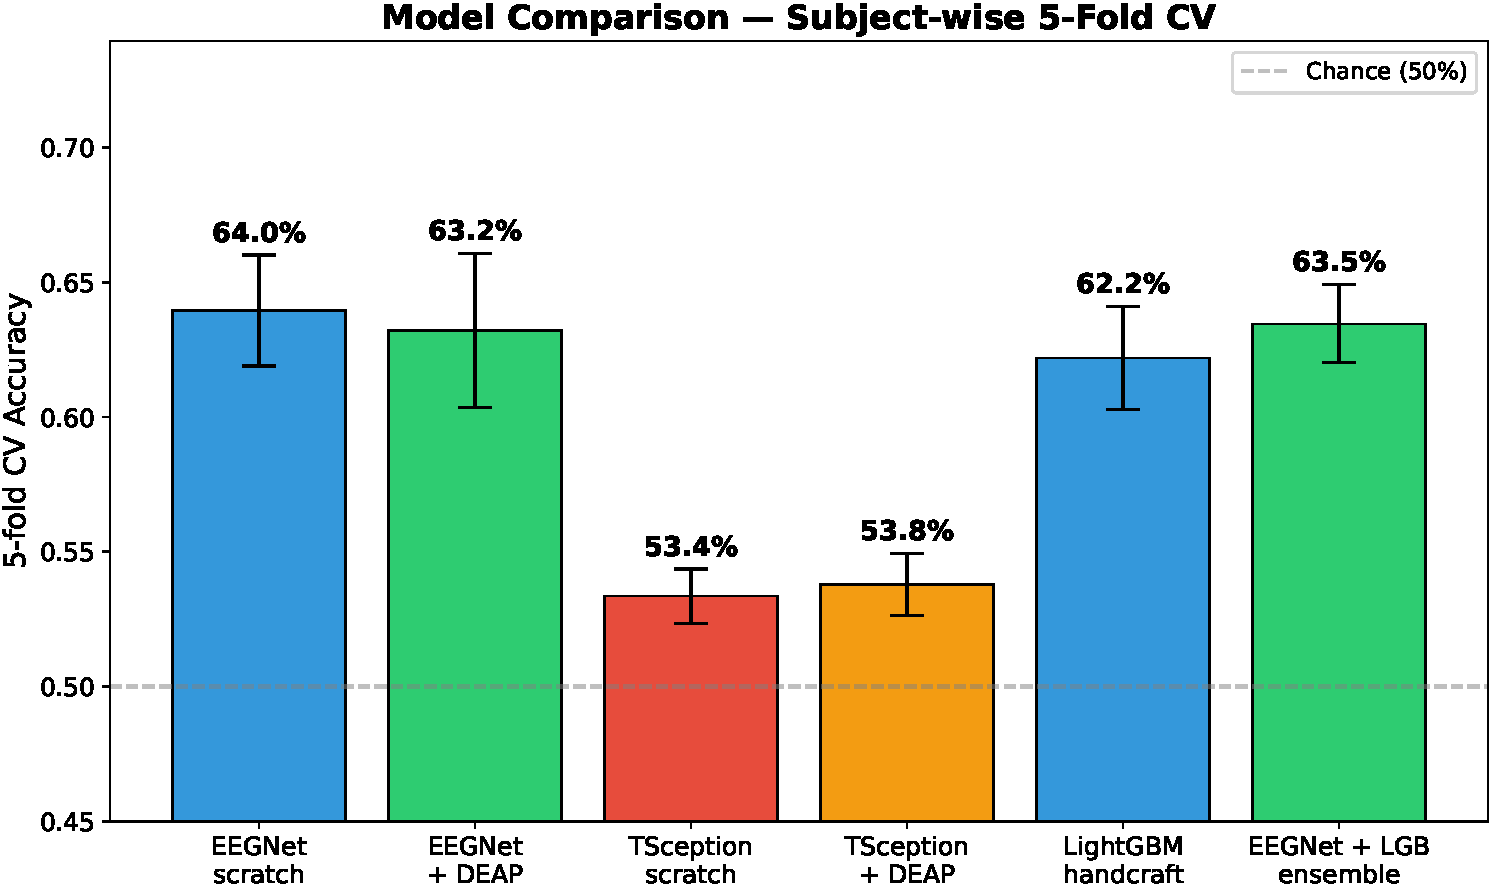
\includegraphics[width=0.75\textwidth]{figures/cv_comparison.pdf}
\caption{各模型5折GroupKFold交叉验证准确率对比}
\label{fig:cv_comparison}
\end{figure}

表\ref{tab:results}给出了全部方法在统一5折GroupKFold划分下的对比结果，图\ref{fig:cv_comparison}以柱状图呈现了各模型准确率的直观对比。六组实验结果从53.35\%到64.26\%不等，最高值与最低值相差约11\%。以下从模型容量、迁移学习和异构融合三个层次展开分析。

首先观察模型容量对泛化性能的影响。TSception和EEGNet同为卷积神经网络，接收完全相同的输入数据并使用完全相同的5折划分进行训练，唯一的差异在架构规模：TSception拥有3,111,106个参数，EEGNet仅有2,834个。两者从零训练的结果分别为53.35\%和63.96\%，准确率相差超过10\%。TSception的53.35\%仅略高于50\%的随机猜测基线，表明该模型在2,400个训练trial的条件下已经过拟合到几乎无法泛化的程度。这是整个对比实验中最关键的发现：在小样本EEG场景中，控制模型容量比架构的精细化设计更为重要。该结论直接验证了方案设计阶段提出的核心假设，即第2.4.2节中引入TSception作为对照的初衷正是为了检验这一容量-泛化关系。

其次考察跨数据集迁移学习的实际效果。DEAP预训练对TSception带来了0.43\%的微弱提升（53.35\%→53.78\%），对EEGNet则反而降低了0.74\%（63.96\%→63.22\%）。两个模型的预训练版本与从零训练版本之间的性能差异均落在各自的标准差范围内，说明DEAP预训练在本实验条件下未产生统计显著的增益。这一"零效果"本身具有信息量：第2.4.2节曾预判DEAP与竞赛数据之间存在采样率（128Hz vs 250Hz）、刺激材料（音乐视频 vs 情绪视频片段）和采集范式三重域鸿沟，实验数据支持了这一预判。需要强调的是，该结果否定的是"任意公开数据集预训练均有益"的朴素假设，而非跨数据集迁移学习本身。在源域与目标域更为接近的条件下（如采用SEED或DREAMER数据集），预训练仍可能带来正面增益。

最后分析异构模型融合的效果。LightGBM（62.19\%）和EEGNet（63.96\%）单独使用时准确率相近，两者差距不足2\%。若两个模型的错误高度重叠，将两者的预测取平均不会带来提升，甚至可能因弱模型的引入而拉低强模型的表现。然而，融合后的准确率达到64.26\%，超出两个单独模型的各自最优值，这表明两者的错误样本集存在显著不重叠：一个模型分错的trial，另一个模型有较大概率分对。第2.5节从数据表示的角度预测了这一互补性（手工特征管线受限于特征框架的完备性，深度学习管线受限于参数空间的表达能力），实验数据构成了对该预测的直接验证。此外，融合模型的标准差（±1.45\%）低于EEGNet（±2.06\%）和LightGBM（±1.91\%），说明软投票融合在提升准确率的同时也降低了跨折预测的波动，增强了模型对被试个体差异的稳健性。

\subsection{消融实验分析}

本方案依次考察预训练、模型容量和手工特征三个关键组件。

\subsubsection{预训练效果消融}

本方案在设计阶段引入DEAP预训练的动机是明确的：竞赛数据仅有60名被试，任何深度学习模型从随机初始化开始训练都面临数据不足的困境；DEAP提供了约30,336个trial，若预训练所学的EEG时空表征能够迁移至竞赛数据，微调阶段的过拟合风险将显著降低。但这一推理隐含了一个关键前提：源域（DEAP）与目标域（竞赛数据）的EEG信号分布必须足够接近，否则预训练权重不仅不能帮助微调，还可能将模型引导至与目标域无关的局部最优点，产生负迁移。

为检验上述前提是否成立，本消融以完全对称的方式对比了两种模型（TSception和EEGNet）在"随机初始化"和"DEAP预训练+微调"两种条件下的5折GroupKFold表现，两组实验使用完全相同的5折划分、相同的优化器配置、相同的早停条件，唯一的变量是训练开始时的权重来源。这一对称设计排除了数据划分或超参数差异对结果的混淆。

两种可能的消融结果分别对应不同的科学结论。若预训练带来显著提升，则验证了跨数据集迁移学习在本任务中的有效性，后续可通过引入SEED等更多公开数据集进一步放大增益。若预训练效果不显著，则说明源域与目标域之间的域鸿沟已超出当前迁移策略的跨越能力，后续工作的方向应转向寻找与竞赛数据更接近的源域，而非简单地增加预训练数据量。

实验结果支持了后者。TSception在加入DEAP预训练后准确率从53.35\%变为53.78\%（+0.43\%），EEGNet从63.96\%变为63.22\%（−0.74\%）。两个变化量的绝对值均小于各自模型的标准差（TSception ±0.84\%，EEGNet ±2.06\%/\allowbreak±2.87\%），在统计意义上无法与零区分。这一消融的结果不是"迁移学习无效"，而是划定了迁移学习在脑电情绪识别中的一个具体边界：当源域和目标域在采样率（128Hz vs 250Hz）、刺激材料（音乐视频 vs 情绪视频片段）和采集范式三个维度同时存在差异时，直接进行模型权重迁移不足以产生可测量的正面增益。该结论为后续工作提供了明确的改进方向：优先缩小源域与目标域的物理参数差异（如选择同为250Hz采样率的SEED数据集），而非在现有DEAP预训练基础上进行增量调参。

\begin{table}[H]
\centering
\caption{预训练效果消融数据}
\label{tab:ablation_pretrain}
\begin{tabular}{lccc}
\toprule
\textbf{模型} & \textbf{训练方式} & \textbf{5折准确率} & \textbf{变化量} \\
\midrule
\multirow{2}{*}{TSception} & 从零训练 & 53.35\% $\pm$ 0.84\% & \multirow{2}{*}{+0.43\%} \\
                           & DEAP预训练+微调 & 53.78\% $\pm$ 0.84\% & \\
\midrule
\multirow{2}{*}{EEGNet}    & 从零训练 & 63.96\% $\pm$ 2.06\% & \multirow{2}{*}{−0.74\%} \\
                           & DEAP预训练+微调 & 63.22\% $\pm$ 2.87\% & \\
\bottomrule
\end{tabular}
\end{table}

\begin{figure}[H]
\centering
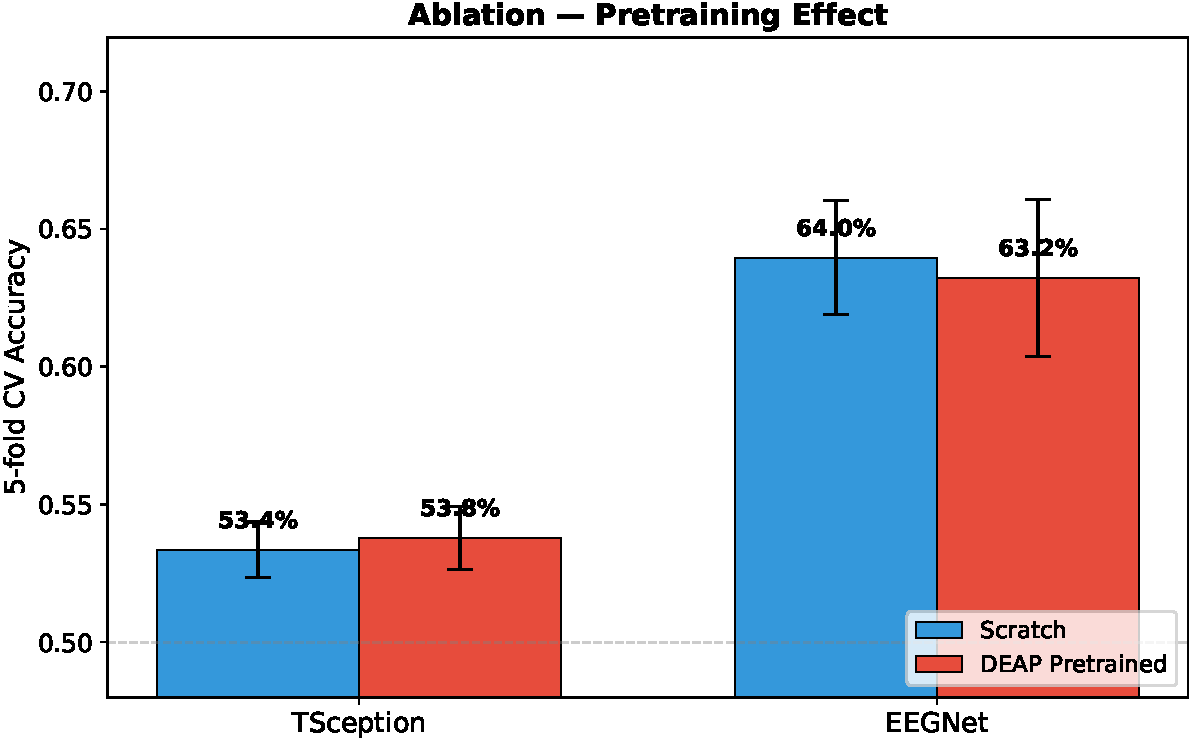
\includegraphics[width=0.65\textwidth]{figures/ablation_pretraining.pdf}
\caption{预训练效果消融：TSception与EEGNet在随机初始化与DEAP预训练后微调两种条件下的5折交叉验证准确率}
\label{fig:ablation_pretrain}
\end{figure}

\subsubsection{模型容量消融}

方案设计阶段提出了一项核心判断：在小样本EEG场景下，模型容量的控制比架构的精细化设计更为关键。这一判断如果成立，意味着在选择模型时，参数量应被置于与特征提取能力同等甚至更高的优先级；如果不成立，则说明精心设计的归纳偏置（如TSception的多尺度时间卷积和半球不对称空间编码）可以弥补参数冗余带来的过拟合风险。验证该判断需要一组对照实验，其中模型容量是唯一的变量，其余所有条件保持恒定。

TSception（3,111,106参数）和EEGNet（2,834参数）恰好构成满足上述要求的对照：两者均为专为脑电解码设计的卷积网络，输入相同的预处理后EEG trial，使用相同的5折划分和相同的训练配置（优化器、学习率调度、早停条件），仅在参数量上相差约1,100倍。这种极端容量差距下的对比不是为了判定TSception和EEGNet两个具体模型的优劣，而是为了回答一个更一般的问题：当训练样本量被固定在约2,400个trial时，将模型容量从数千参数推高至数百万参数，泛化性能会如何变化。

实验给出的答案是明确且反直觉的。EEGNet以2,834参数取得63.96\%的准确率，TSception以3,111,106参数仅取得53.35\%，容量更大的模型反而低了10\%以上。这一方向与传统深度学习"容量越大表征能力越强"的经验相反，但恰好印证了方案设计阶段的预判：当数据量不足以支撑高维参数空间的可靠估计时，模型会将训练集中与情绪无关的噪声模式也纳入拟合目标，导致在未见过的被试上泛化失败。TSception微调过程中的训练曲线（图\ref{fig:finetune}）提供了直接的过拟合证据：训练准确率随epoch持续上升而验证准确率停滞甚至下降，两条曲线之间不断扩大的差距正是模型在噪声中拟合的典型特征。

该消融的工程含义是明确的：在本实验条件下（60人、2,400 trial），不应为了追求架构的表征能力而放松对参数量的控制。EEGNet的2,834参数并非"越少越好"的极端，而是模型容量与数据规模之间的一个可行匹配点。该结论同时提示，若未来能通过增加被试或引入更接近的源域预训练来有效扩大训练数据规模，TSception等较大模型的表现可能得到改善：容量本身不是问题，容量与数据量的比值才是。

\begin{table}[H]
\centering
\caption{模型容量消融数据}
\label{tab:ablation_capacity}
\begin{tabular}{lccc}
\toprule
\textbf{模型} & \textbf{参数量} & \textbf{5折准确率} & \textbf{训练时间} \\
\midrule
TSception & 3,111,106 & 53.35\% $\pm$ 0.84\% & $\sim$2h \\
EEGNet    & 2,834     & 63.96\% $\pm$ 2.06\% & $\sim$3min \\
\bottomrule
\end{tabular}
\end{table}

\begin{figure}[H]
\centering
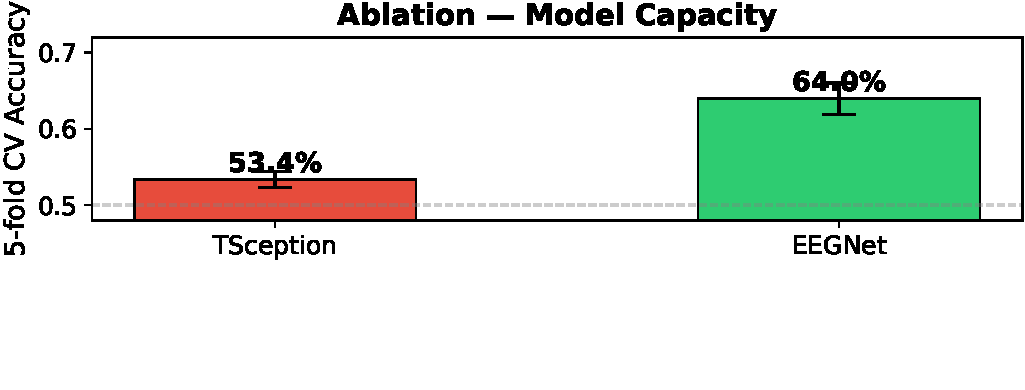
\includegraphics[width=0.55\textwidth]{figures/ablation_capacity.pdf}
\caption{模型容量消融：TSception与EEGNet从零训练的5折交叉验证准确率，二者参数量相差约1,100倍}
\label{fig:ablation_capacity}
\end{figure}

\subsubsection{手工特征贡献分析}

前两项消融针对深度学习管线，第三项分析转向手工特征管线。与前两项通过移除组件来观测性能变化不同，本项分析的目标是在390维特征空间内部识别信息密度的分布，即哪些频段和通道的组合对情绪分类的贡献最大。该问题的工程意义在于指导特征精简（若少数特征承载了大部分信息，则可压缩特征维度以进一步降低过拟合风险），其神经科学意义在于提供独立的数据驱动证据来检验模型是否收敛到已知的情绪神经机制上。

特征重要性的量化使用LightGBM内置的split gain指标。决策树的每次分裂选择一个特征的一个阈值将当前节点样本分为两组，分裂前后分类损失函数的下降量即为该次分裂的增益。同一特征在所有决策树的所有分裂中产生的增益之和构成该特征的总增益，直接反映该特征对模型全局决策的累计贡献。增益计算在训练过程中自动完成，无需额外的统计检验。

图\ref{fig:feature_importance}和表\ref{tab:feature_importance}给出了增益排名前15的特征，两个规律跨频段和跨通道地一致呈现。在频段维度上，微分熵（DE）特征占据了前15位中的13席，功率谱密度（PSD）和Hjorth参数各占1席。DE内部呈现出清晰的频段集中：$\gamma$波段（31--50Hz）DE特征7席，$\alpha$波段（8--14Hz）DE特征2席，其余频段的DE分布稀疏。$\gamma$波段DE的主导地位与Duan等在公开数据集上的系统特征比较结论一致\cite{duan_de}，表明这一频段-特征组合的判别优势具有一定的跨数据集泛化性。$\alpha$波段DE的高贡献则与前额叶$\alpha$不对称理论中效价与$\alpha$功率的关联方向一致\cite{coan}。

在空间维度上，排名前15的特征涉及的通道呈现明显的区域性聚集：通道18、12、17、22和27反复出现，这些电极在国际10--20系统中集中分布于顶叶中央区与后颞区的交界处\cite{ten_twenty}。该区域在功能神经成像文献中与情绪刺激的躯体感觉加工和自主神经唤醒成分相关。值得注意的是，特征重要性排序完全由数据驱动，模型未接受任何关于电极空间位置的先验信息。数据自动筛选出的高贡献通道恰好落在一个具有已知神经科学意义的脑区，这一独立一致性降低了模型仅拟合数据噪声的可能性。

上述频段和通道的双重收敛对后续工作具有实用价值：若需在更受限的硬件条件下部署模型，可优先保留$\gamma$和$\alpha$波段DE以及通道18、12、17、22、27对应电极的数据，以远小于390维的特征量级维持分类性能的主体部分。

\begin{table}[H]
\centering
\caption{LightGBM特征重要性Top-15（split gain累计值）}
\label{tab:feature_importance}
\begin{tabular}{lcl@{\hspace{1.5cm}}lcl}
\toprule
\textbf{排名} & \textbf{特征名称} & \textbf{增益值} &
\textbf{排名} & \textbf{特征名称} & \textbf{增益值} \\
\midrule
1  & DE\_gamma\_18  & 47 & 9  & DE\_gamma\_13  & 18 \\
2  & DE\_gamma\_12  & 32 & 10 & DE\_gamma\_22  & 16 \\
3  & DE\_gamma\_17  & 30 & 11 & Hjorth\_mob\_18 & 16 \\
4  & Hjorth\_comp\_22 & 23 & 12 & PSD\_gamma\_18 & 15 \\
5  & DE\_alpha\_27  & 22 & 13 & DE\_gamma\_23  & 15 \\
6  & DE\_gamma\_27  & 20 & 14 & Hjorth\_mob\_6  & 14 \\
7  & DE\_beta\_3    & 19 & 15 & PSD\_gamma\_17 & 14 \\
8  & DE\_alpha\_13  & 19 &    &                &    \\
\bottomrule
\end{tabular}
\end{table}

\begin{figure}[H]
\centering
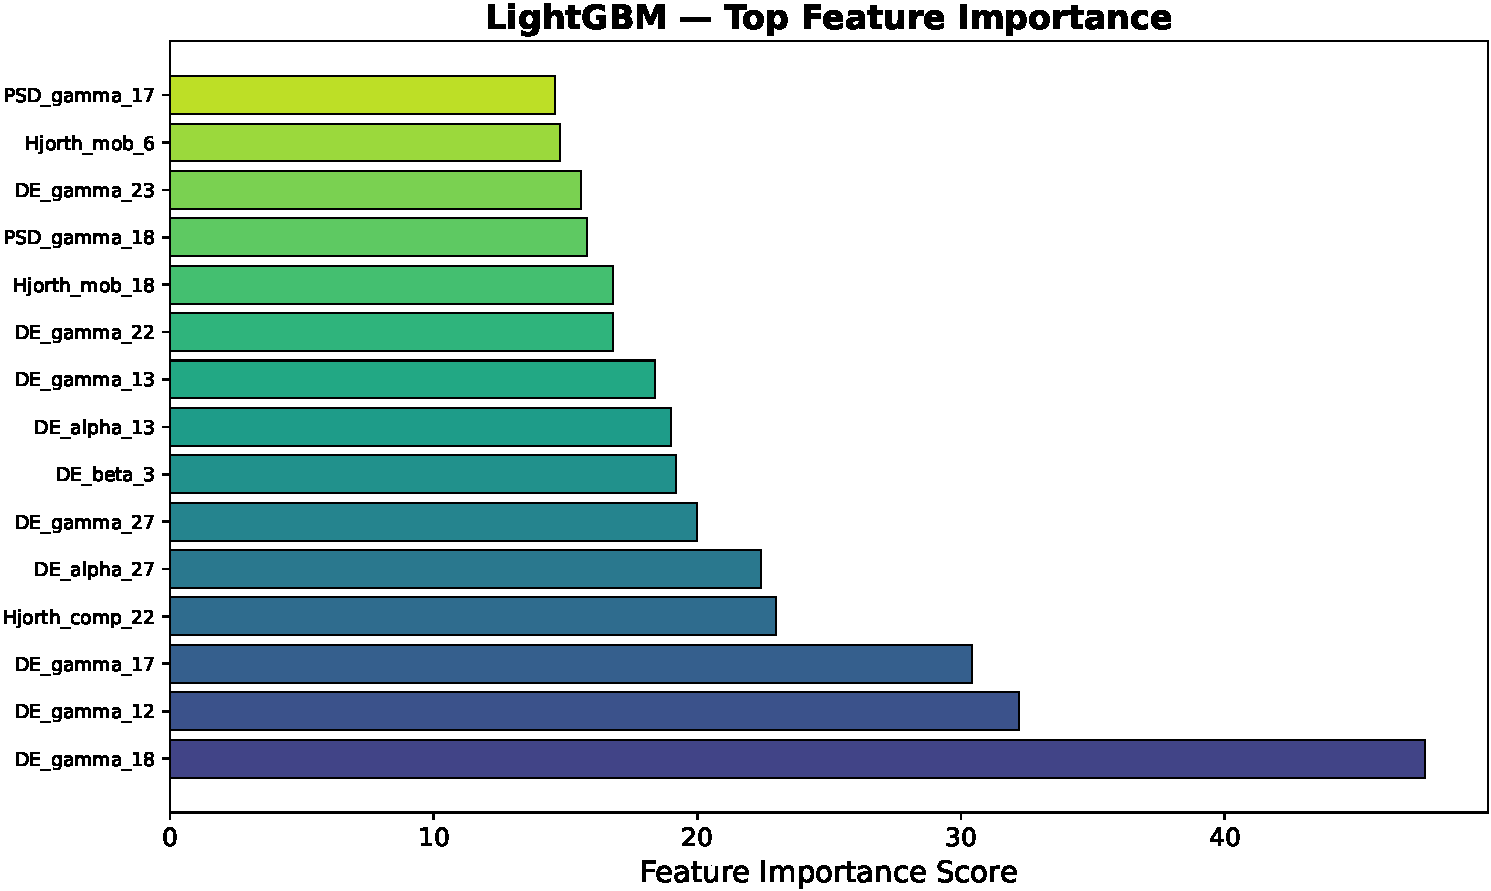
\includegraphics[width=0.75\textwidth]{figures/feature_importance.pdf}
\caption{LightGBM特征重要性Top-15可视化}
\label{fig:feature_importance}
\end{figure}

\subsection{训练过程分析}

\begin{figure}[H]
\centering
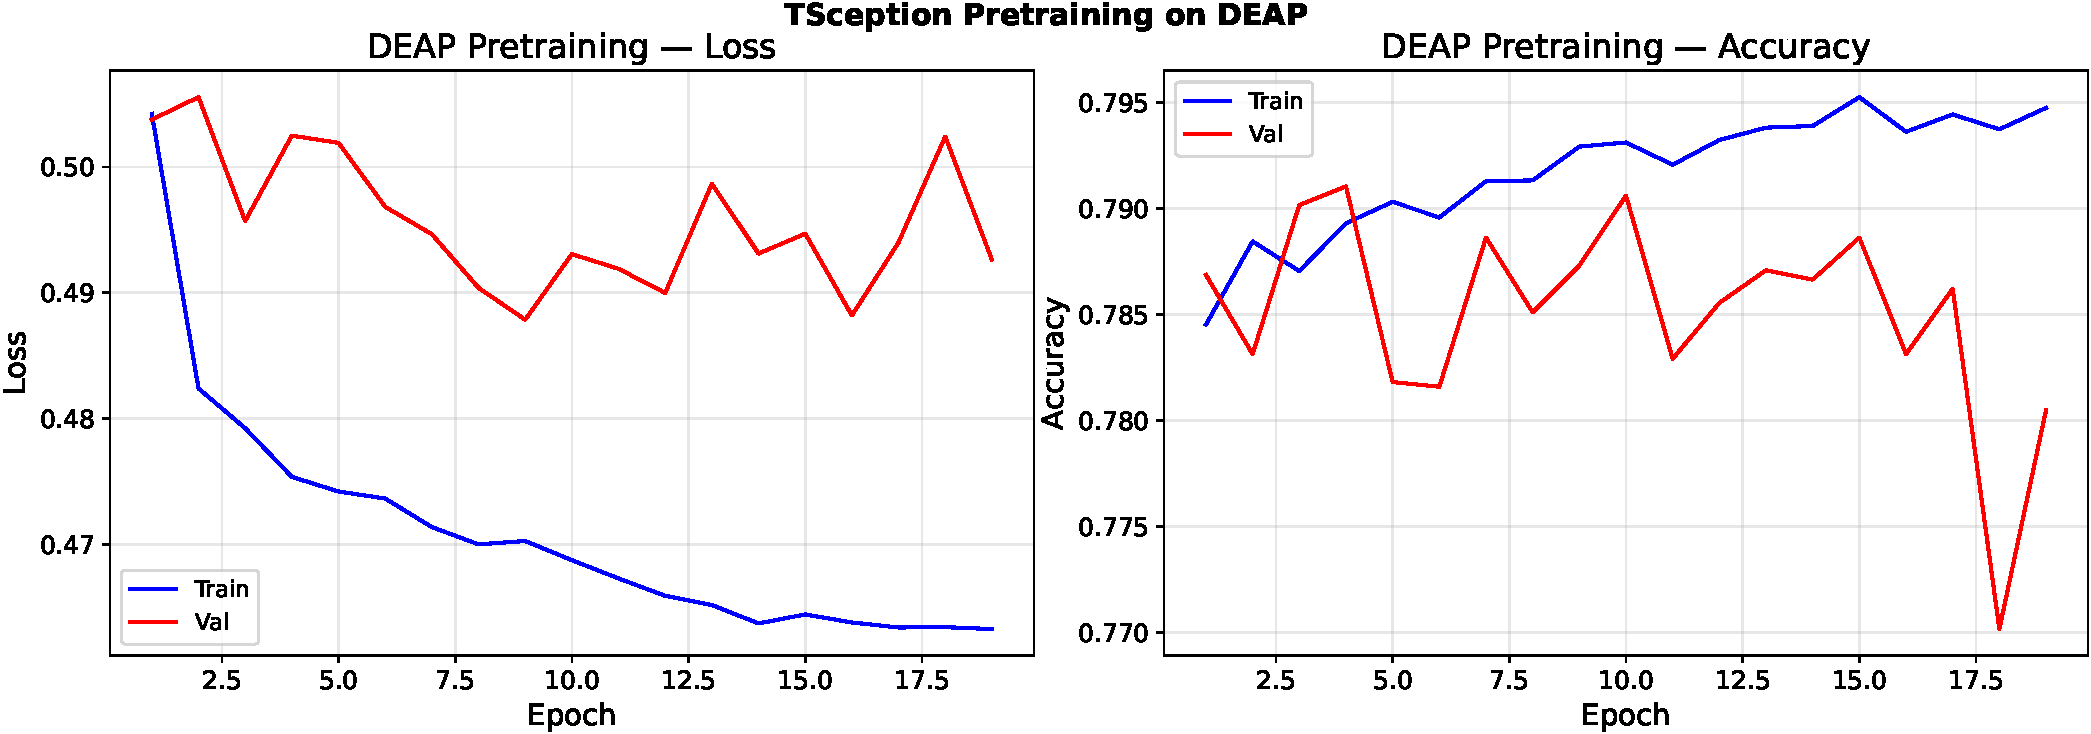
\includegraphics[width=0.75\textwidth]{figures/pretrain_curves.pdf}
\caption{DEAP预训练过程中EEGNet的训练与验证曲线}
\label{fig:pretrain}
\end{figure}

EEGNet在DEAP预训练过程中仅用1.8分钟训练19个epoch即达到79.10\%验证准确率，早停机制在验证损失不再下降时自动终止训练。微调阶段的训练曲线（图\ref{fig:finetune}）显示，EEGNet验证准确率在16个epoch左右趋于平稳，无明显过拟合现象；而TSception在微调过程中训练准确率持续上升但验证准确率停滞，表现出典型的过拟合特征。

\begin{figure}[H]
\centering
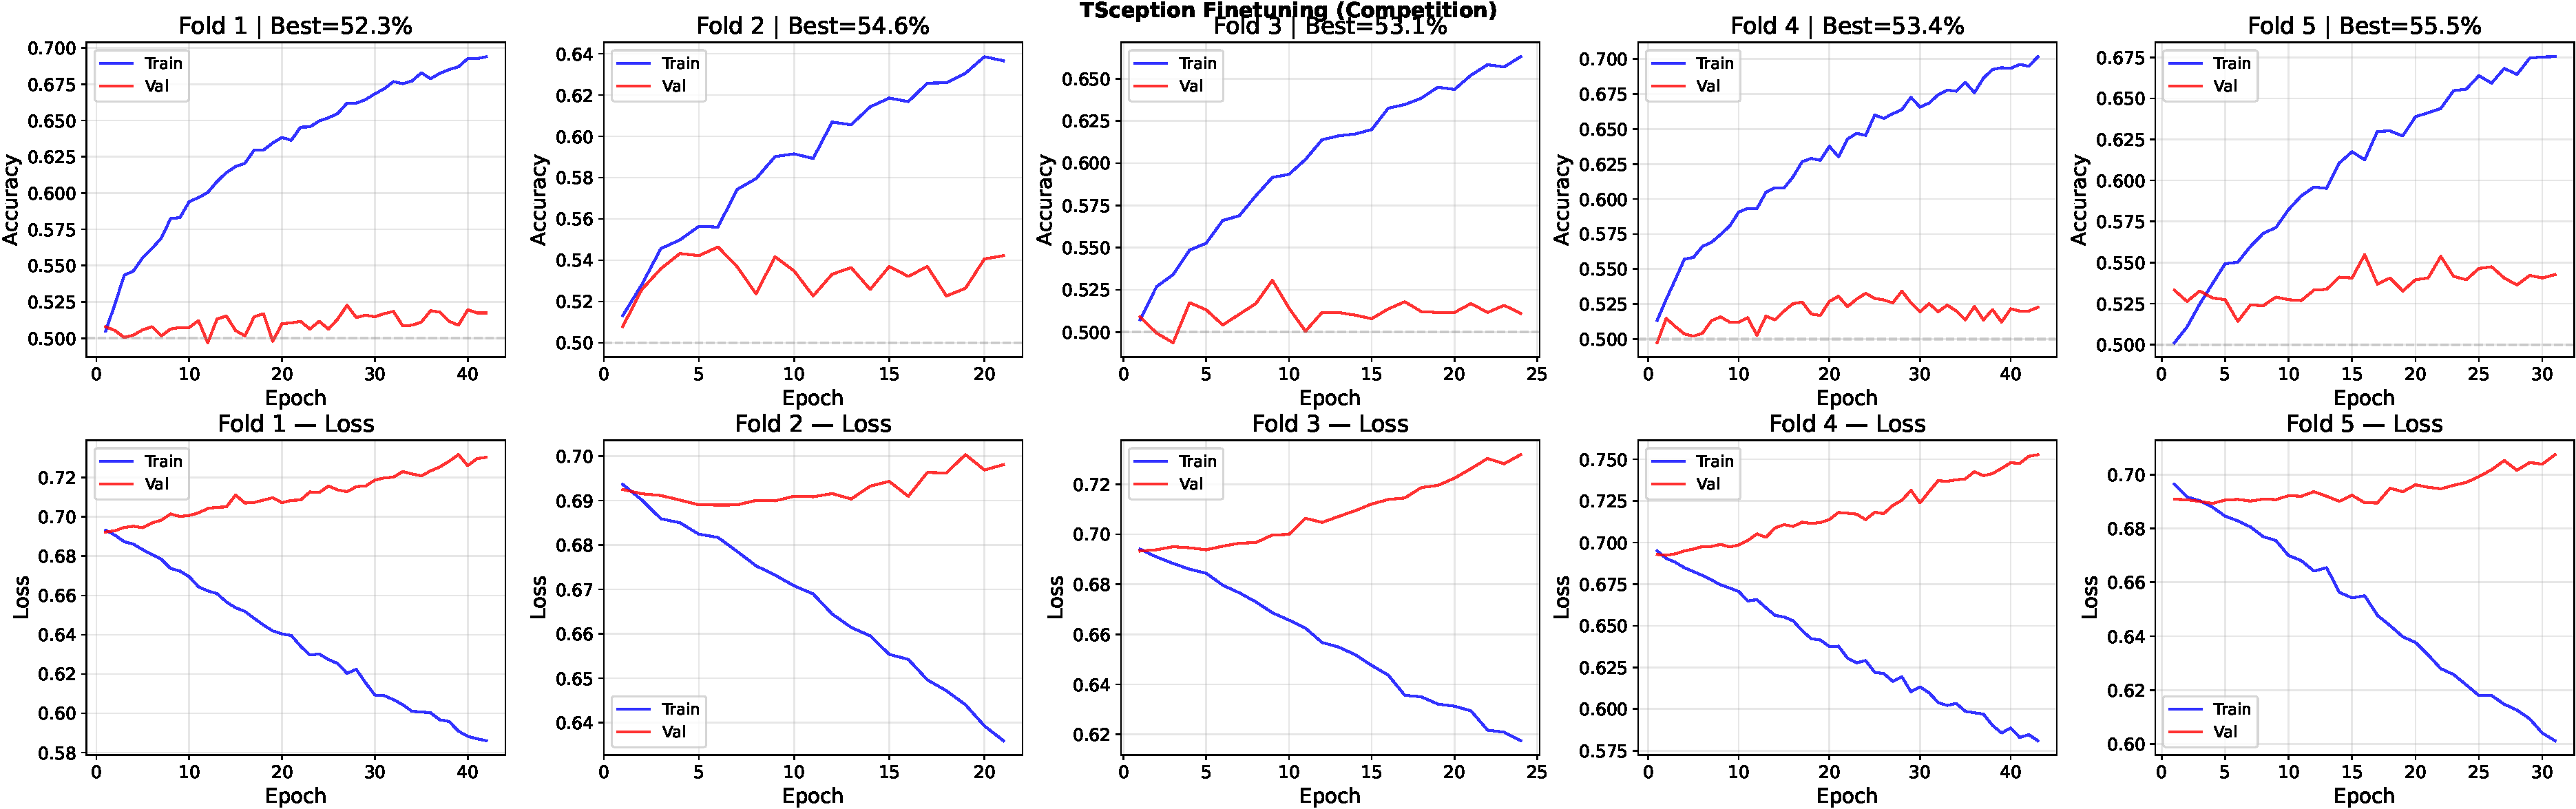
\includegraphics[width=0.75\textwidth]{figures/finetune_folds.pdf}
\caption{EEGNet在竞赛数据上5折微调的训练与验证曲线}
\label{fig:finetune}
\end{figure}

\subsection{测试集推理}

基于最终测试方案，使用EEGNet + LightGBM融合模型对10名测试被试的脑电数据进行推理预测。测试数据按官方描述，每名被试包含8段情绪视频对应的10秒脑电片段（共80个trial），预测结果以规定模板格式输出为submission.xlsx文件。

% =================================================================
% 第 4 章：总结
% =================================================================
\section{总结}

\subsection{核心技术成果}

本文围绕小样本脑电情绪识别中的过拟合与跨被试泛化两大难题，构建了深度迁移学习与手工特征融合的双管线方案。在数据层面，竞赛数据与DEAP公开数据经统一的0.5--50Hz带通滤波、10秒分段和Z-score标准化处理后，形成格式对齐的训练与预训练数据集。在特征层面，微分熵、功率谱密度和Hjorth参数三类共计390维手工特征将75,000维的原始信号空间压缩至390维，在保留已知情绪相关频域和时域信息的同时使下游分类器的统计学习成为可能。在模型层面，轻量级EEGNet（2,834参数）和大容量TSception（3,111,106参数）构成了一组容量-泛化关系的对照实验，手工特征与LightGBM的组合构成第二条独立管线，两条管线的软投票融合构成第三条路径。在验证层面，所有实验在5折GroupKFold按被试划分的策略下评估，以确保验证分数反映模型对陌生被试的泛化能力。实验结果表明：轻量级模型的泛化性能显著优于大容量模型（63.96\% vs 53.35\%），手工特征管线达到62.19\%，异构融合达到最高的64.26\%。DEAP预训练未产生统计显著的增益，其根源在于源域与目标域在采样率、刺激材料和采集范式上的三重差异。特征重要性分析独立地识别出$\gamma$和$\alpha$波段微分熵以及顶颞区电极（通道18、12、17、22）为情绪分类的核心特征和通道，与神经科学文献形成独立一致。

\subsection{算法设计的创新性}

本方案在方法层面的贡献不在于提出全新的算法架构，而在于通过系统的实验设计回答了小样本脑电情绪识别中的三个递进问题。

一是模型容量的边界。将TSception和EEGNet置于完全相同的输入、划分和训练条件下进行对比，二者参数量相差约1,100倍，构成了一个天然的容量消融实验。实验结论（容量更大的模型反而准确率低10\%以上）并非对TSception架构的否定，而是以量化方式界定了当前数据规模（60人，约2,400 trial）下模型容量的合理范围。这一发现对后续工作具有直接的工程参考价值：在数据规模未显著扩大的前提下，优先选择参数量与数据量匹配的轻量级架构。

二是迁移学习的边界。DEAP预训练在两个模型上均未产生可测量的正面增益，这一"零结果"本身提供了明确的信息：当源域与目标域在采样率、刺激模态和采集范式上同时存在显著差异时，直接进行模型权重迁移的有效性受限。该结论将迁移学习的讨论从"是否有效"聚焦到"何种条件下有效"，为后续源域的选择提供了具体标准。

三是异构模型互补的验证。手工特征管线和深度学习管线在数据表示（390维结构化特征 vs 原始波形）和学习机制（梯度提升树 vs 卷积网络）上完全不同，两种模型在GroupKFold验证中的错误样本集存在显著不重叠，软投票融合后准确率超出两个单独模型。该结果以实验方式验证了"不同学习范式的错误模式具有互补性"这一假设。

\subsection{方案与模型的完整性}

本文构建的脑电情绪识别管线覆盖了从原始数据到最终分类决策的完整链路。预处理阶段，竞赛数据与DEAP数据经过统一的通道对齐、带通滤波、滑动窗分段和Z-score标准化，两条数据管线在频域条件和信号统计特性上保持一致，为后续的跨数据集迁移学习提供了统一的数据基础。特征工程阶段，三类手工特征分别覆盖频域能量（PSD）、频域统计结构（DE）和时域波形形态（Hjorth参数），从三个互补的视角提取情绪相关的脑电信息，合计390维。模型训练阶段，并行构建了手工特征+LightGBM和原始信号+EEGNet两条管线，并设置了TSception作为容量对照、DEAP预训练+微调作为迁移学习对照。验证阶段，通过预训练效果消融、模型容量消融和特征贡献分析三项消融实验，逐组件量化了每个设计决策的边际效应。全流程代码从数据预处理、特征提取、模型训练、交叉验证到测试集推理均可复现运行。

\subsection{本地可验证的性能}

性能评估建立在严格的跨被试验证框架之上。采用5折GroupKFold按被试划分策略，划分的原子单位是被试而非trial，确保同一被试的数据不会被拆分至训练集和验证集两侧。全部对比方法使用完全相同的5折随机划分（固定随机种子），排除了数据划分差异对方法间比较的干扰。

在该验证框架下，六组方法在5折CV中的平均准确率范围为53.35\%至64.26\%。各方法的跨折标准差在0.84\%至2.87\%之间，反映了模型在不同被试组上的性能波动幅度。融合模型的标准差（±1.45\%）低于两个单独模型（EEGNet ±2.06\%，LightGBM ±1.91\%），表明融合策略在提升准确率的同时也增强了跨被试的稳定性。训练过程的收敛曲线（图\ref{fig:pretrain}、图\ref{fig:finetune}）显示EEGNet在预训练和微调阶段均正常收敛，未出现训练-验证曲线显著分离的过拟合特征；而TSception的曲线则出现了训练准确率持续上升、验证准确率停滞的典型过拟合模式，与容量消融的结论相互印证。

\subsection{展望}

本工作揭示了若干有待进一步探索的方向。在预训练数据方面，DEAP与竞赛数据之间的域鸿沟限制了迁移学习的收益，引入SEED、DREAMER等在采样率和采集范式上更接近竞赛数据的公开数据集，有望突破当前预训练策略的性能瓶颈。在模型架构方面，STAFNet\cite{stafnet}、DAMGCN等集成了注意力机制和图神经网络的最新架构在公开数据集上取得了领先性能，但其参数量通常较高，在小样本场景下的适用性需配合针对性的正则化和容量控制策略进行验证。在可解释性方面，Grad-CAM和SHAP等方法可将模型的时间-空间关注区域可视化，为特征重要性分析提供更细粒度的补充证据。在训练范式方面，自监督对比学习可利用大规模无标注脑电数据预训练表征编码器，降低对有标注数据的依赖，在脑电情绪识别领域具有潜在的应用前景。

% =================================================================
% 参考文献
% =================================================================
\phantomsection
\addcontentsline{toc}{section}{参考文献}
\begin{thebibliography}{99}

\bibitem{eegnet}
Lawhern, V.J. et al. (2018). EEGNet: A Compact Convolutional Neural Network for EEG-based Brain-Computer Interfaces. \textit{Journal of Neural Engineering}.

\bibitem{tsception}
Ding, Y. et al. (2023). TSception: Capturing Temporal Dynamics and Spatial Asymmetry from EEG for Emotion Recognition. \textit{IEEE Transactions on Affective Computing}.

\bibitem{deap}
Koelstra, S. et al. (2012). DEAP: A Database for Emotion Analysis Using Physiological Signals. \textit{IEEE Transactions on Affective Computing}.

\bibitem{lightgbm}
Ke, G. et al. (2017). LightGBM: A Highly Efficient Gradient Boosting Decision Tree. \textit{NeurIPS}.

\bibitem{ten_twenty}
Klem, G.H. et al. (1999). The Ten-Twenty Electrode System of the International Federation. \textit{Electroencephalography and Clinical Neurophysiology}, 52(3): 3--6.

\bibitem{eeg_preprocessing}
Bigdely-Shamlo, N. et al. (2015). The PREP Pipeline: Standardized Preprocessing for Large-Scale EEG Analysis. \textit{Frontiers in Neuroinformatics}, 9: 16.

\bibitem{butterworth}
Butterworth, S. (1930). On the Theory of Filter Amplifiers. \textit{Experimental Wireless and the Wireless Engineer}, 7: 536--541.

\bibitem{duan_de}
Duan, R.N., Zhu, J.Y., Lu, B.L. (2013). Differential Entropy Feature for EEG-based Emotion Classification. \textit{Proceedings of the 6th International IEEE/EMBS Conference on Neural Engineering (NER)}, 81--84.

\bibitem{coan}
Coan, J.A. and Allen, J.J.B. (2004). Frontal EEG Asymmetry as a Moderator and Mediator of Emotion. \textit{Biological Psychology}, 67(1--2): 7--50.

\bibitem{welch}
Welch, P.D. (1967). The Use of Fast Fourier Transform for the Estimation of Power Spectra. \textit{IEEE Transactions on Audio and Electroacoustics}, 15(2): 70--73.

\bibitem{hjorth}
Hjorth, B. (1970). EEG Analysis Based on Time Domain Properties. \textit{Electroencephalography and Clinical Neurophysiology}, 29(3): 306--310.

\bibitem{stafnet}
Hu, X. et al. (2024). STAFNet: An Adaptive Multi-Feature Learning Network via Spatiotemporal Fusion for EEG-based Emotion Recognition. \textit{Frontiers in Neuroscience}.

\end{thebibliography}

\end{document}
